\documentclass[12pt]{ucsddissertation}
% mathptmx is a Times Roman look-alike (don't use the times package)
% It isn't clear if Times is required. The OGS manual lists several
% "standard fonts" but never says they need to be used.
\usepackage{mathptmx}
\usepackage[NoDate]{currvita}
\usepackage{array}
\usepackage{tabularx}
\usepackage{booktabs}
\usepackage{ragged2e}
\usepackage{microtype}
\usepackage[breaklinks=true,pdfborder={0 0 0}]{hyperref}
\usepackage{graphicx}
\AtBeginDocument{%
	\settowidth\cvlabelwidth{\cvlabelfont 0000--0000}%
}

% OGS recommends increasing the margins slightly.
\increasemargins{.1in}

% These are just for testing/examples, delete them
\usepackage{trace}
%\usepackage{showframe} % This package was just to see page margins
\usepackage[english]{babel}
\usepackage{blindtext}
\overfullrule5pt
% ---

% Required information
\title{Understand Threat Intelligence: Data, Operation and Threat Landscape}
\author{Guo Li}
\degree{Computer Science}{Doctor of Philosophy}
% Each member of the committee should be listed as Professor Foo Bar.
% If Professor is not the correct title for one, then titles should be
% omitted entirely.
\cochair{Professor Stefan Savage}
\cochair{Professor Kirill Levchenko}
% Your committee members (other than the chairs) must be in alphabetical order
\committee{Professor Geoffrey M. Voelker}
\committee{Professor Deian Stefan}
\committee{Professor Xinyu Zhang}
\degreeyear{2020}

% Start the document
\begin{document}
% Begin with frontmatter and so forth
\frontmatter
\maketitle
\makecopyright
\makesignature
% Optional
\begin{dedication}
\setsinglespacing
\raggedright % It would be better to use \RaggedRight from ragged2e
\parindent0pt\parskip\baselineskip
In recognition of reading this manual before beginning to format the
doctoral dissertation or master's thesis; for following the
instructions written herein; for consulting with OGS Academic Affairs
Advisers; and for not relying on other completed manuscripts, this
manual is dedicated to all graduate students about to complete the
doctoral dissertation or master's thesis.

In recognition that this is my one chance to use whichever
justification, spacing, writing style, text size, and/or textfont that
I want to while still keeping my headings and margins consistent.
\end{dedication}
% Optional
\begin{epigraph}
\vskip0pt plus.5fil
\setsinglespacing
{\flushright
True ease in writing comes from art, not chance,\\
As those move easiest who have learn'd to dance.\\
'T is not enough to no harshness gives offence,---\\
The sound must seem an echo to the sense.

\vskip\baselineskip
\textit{Alexander Pope}\par}
\vfil
\begin{center}
You write with ease to show your breeding,\\
But easy writing's curst hard reading.

\vskip\baselineskip
\textit{Richard Brinsley Sheridan}
\end{center}
\vfil
\noindent Writing, at its best, is a lonely life. Organizations for
writers palliate the writer's loneliness, but I doubt if they improve
his writing. He grows in public stature as he sheds his loneliness and
often his work deteriorates. For he does his work alone and if he is a
good enough writer he must face eternity, or the lack of it, each day.

\vskip\baselineskip
\hskip0pt plus1fil\textit{Ernest Hemingway}\hskip0pt plus4fil\null

\vfil
\end{epigraph}

% Next comes the table of contents, list of figures, list of tables,
% etc. If you have code listings, you can use \listoflistings (or
% \lstlistoflistings) to have it be produced here as well. Same with
% \listofalgorithms.
\tableofcontents
\listoffigures
\listoftables

% Preface
\begin{preface}
Almost nothing is said in the manual about the preface. There is no
indication about how it is to be typeset. Given that, one is forced to
simply typeset it and hope it is accepted. It is, however, optional
and may be omitted.
\end{preface}

% Your fancy acks here. Keep in mind you need to ack each paper you
% use. See the examples here. In addition, each chapter ack needs to
% be repeated at the end of the relevant chapter.
\begin{acknowledgements}
First and foremost, I would like to thank my advisors, professor Stefan
Savage and professor Kirill Levchenko. When I first joined the PhD program,
I was an introvert student with little understanding of research. I was
too scared to try something new or to think boldly. Thanks to my advisors,
who both have very clean visions and are not afraid to take risks, I had a 
very wild PhD experience. We tried a completely new idea for malware 
analysis, reverse-engineered Volkswagen engine firmware to try to disclose 
its cheating logic, and eventually moved to Threat Intelligence and try to 
picture the landscape of threat on the Internet. Some projects worked out, 
some did not, but I learned so much from this journey. They taught me
to always follow my interests, not the trend, and never be afraid of 
failure. This attitude towards research had changed me a lot, both in the
way of doing research, also in the way of making life decisions. Besides, 
I really appreciate that both of my advisors gave me great freedom during
my study, which makes my PhD journey a lot less stressful, and at the same 
time taught me to be independent very early on.

I also liked to thank professor Geoffrey M. Voelker. Although he is not my
official advisor, he helped me a lot during two of my projects, both of 
which are covered in this dissertation. He also gave me a lot of valuable 
guidance during some of my lowest points. I really thank his kindness
and caring. I would also like to thank Professors Deian Stefan and Xinyu Zhang 
for being on my doctoral committee and being available whenever I needed help.

PhD experience is fun but also challenging, and I can not make it 
without the help from so many people, especially from my ``Foundry'' lab
mates (CSE 3142), where everyone is so kind and supportive.
Our lab has a very free, open atmosphere, and we discuss almost anything
freely here. With these discussions and exchange of ideas, I become 
more objective on thinking, and learned a lot on many different 
topics. We are also hard-working and spent many long nights together
at lab. I will never forget those times when we laugh and fight together. 
I would also like to thank members from ``Tiger'' lab (CSE 3152), we 
hang out frequently and give support to each other during hard times. The style 
of how they approach research problems---being very strict on defining the
problem and validating with real-world examples---inspired me a lot.

Special thanks to Danny Huang and Tianyin Xu. These two senior students(now 
both become professors) had helped me a lot during my PhD and give me
valuable advice. During my lowest points, I had multiple long conversations
with them, and they shared a lot of their own stories and encouraged me to
keep going. Their encouragement and the experience they shared is critical 
for my journey.

I would like than all the member of Sysnet group, including all the faculties,
staffs and students. It has been a wonderful 6 years for me, and I had many 
interactions with many people during this process, in security lunch, 
syslunch, sysnet hiking, CNS meeting etc. All these activities not only enable
me to learn a lot of stuff, but also make my journey much more enjoyable, and 
give me a strong feeling of belonging. Special thanks to Cindy Moore, who 
helped me numerous times setting up servers and fixing network issues. 

Chapter~\ref{chapter:data_character}, in part, is a reprint of the material 
as it appears in Proceedings of the Usenix Security 2019. \textit{Reading the 
Tea Leaves: A Comparative Analysis of Threat Intelligence.} Vector Guo Li,
Matthew Dunn, Paul Pearce, Damon McCoy, Geoffrey M. Voelker, Stefan Savage,
Kirill Levchenko. The dissertation author was the primary investigator and 
author of this paper. I really like to thank my coauthors on this paper,
without who I will never be able to finish this work. I like to especially 
thank Paul Pearce, who helped me a lot throughout the project. At the
beginning, when I had little idea about what to do and was so unfamiliar with 
data analysis tools, he gave me critical hands-on assists. I am also very
grateful to Alberto Dainotti and Alistair King for sharing the UCSD telescope
data and helping me with the analysis, also professor Micheal Bailey for 
sharing the Mirai Botnet data. Besides, I like to thanks professor Aaron 
Schulman, who encouraged me a lot when the first submission of this paper 
was rejected, and helped me regain my confidence in the work.

Chapter~\ref{chapter:data_usage}, in part, is a reprint of the material as 
submitted to the Proceedings of the Usenix Security 2020. \textit{
Clairvoyance: Inferring Blacklist Use on the Internet} Vector Guo Li, 
Gautam Akiwate, Yihui Chen, Geoffrey M. Voelker, Kirill Levchenko, Stefan 
Savage. The dissertation author was the primary investigator and author of 
this paper. I really appreciate the help from my coauthors, especially 
Gautam Akiwate. He helped me a lot on data collection and analysis,
and I really learned a lot from the way he looks at data problems. 
Furthermore, he gave me crucial moral support during some critical times
of the project. I will not be able to finish this work without his help.
I also really appreciate the suggestions I received from kc Claffy and 
Alex Gantman regarding this project.

Last but not least, I want to thank my parents. My parents know little
about research, but they know how to do things. They gave me lots of 
suggestions on my study, but I was too fool to realize how valuable those 
suggestions are. This journey is tough, and many times when I did not
know what to do, when I lost my hope, when I thought about giving up,
they supported me, encouraged me, gave me strength and hope to 
carry on and keep going. If the PhD journey is walking through a dark 
tunnel, then they are the torch in my hand that are always there,
calm me down, show me the way and bring me warmth. They are the source of 
my strength and my motivation to work hard. It is very lucky for me to have 
such wise and supportive parents, and I will never forget their love 
and caring.
\end{acknowledgements}


% Stupid vita goes next
\begin{vita}
\noindent
\begin{cv}{}
\begin{cvlist}{}
\item[2014] Bachelor of Science, Peking University
\item[2014--2020] Research Assistant, University of California, San Diego
\item[2017] Master of Science in Computer Science, University of California, San Diego
\item[2020] Doctor of Philosophy in Computer Science, University of California, San Diego
\end{cvlist}
\end{cv}
\end{vita}

% Put your maximum 350 word abstract here.
\begin{dissertationabstract}

Threat Intelligence, both as a concept and a product, has been increasingly
gaining prominence in the security industry. At a high-level, it is the 
``knowledge'' that helps organizations understand and mitigate cyber-attacks.
Most commonly, it refers to the collection of threat indicators---IP 
addresses, domain names, file hashes, etc. known to be associated with 
attacks. By compiling and distributing this information, it is believed 
that recipients will be able to better 
defend their systems from future attacks. Thus, there are now hundreds of
vendors offering their threat intelligence solutions as a mix of public and
commercial products. 

However, our understanding of this data, its characterization, and the
extent to which it can meaningfully support its intended uses, is
still quite limited. Furthermore, how the data is being used by
organizations, how popular it is, and what impact it could have on the 
Internet are also not clear to our community. We lack an empirical 
assessment of real-world threat intelligence, both in terms of the data
itself and its usage, and it is important to first understand the current 
status of threat intelligence, then can we reasonably discuss how to make
improvements.

In this dissertation, I take an empirical approach to study threat 
intelligence and try to address these gaps. In particular, I explore 
this topic from two perspectives: 1) the characteristic and dynamics of 
threat intelligence data feeds and 2) how they are used in the 
real-world. In particular, I formally defined a set of metrics for 
analyzing threat intelligence data feeds and use these measures to 
systematically characterize a broad range of public and commercial feeds. 
Further, I ground my quantitative assessments using external measurements 
to qualitatively investigate issues of coverage and accuracy. Finally, I
designed a method using the IP ID side channel to test if a remote host 
is blocking traffic from a given IP address. Using this technique, I 
measure over {\reflroughnum} U.S. hosts and test whether they 
consistently block connections with IPs identified on popular IP blacklists. 
Beyond these blacklists, I also demonstrate the evidence for more widespread 
use of other blacklists for traffic blocking. Together, my work provides
an in-depth look into the current picture of threat intelligence and augments
the knowledge of our community on this topic.

\end{dissertationabstract}


% This is where the main body of your dissertation goes!
\mainmatter

% Optional Introduction
% Optional Introduction
\chapter{Introduction}

Computer security is an inherently adversarial discipline in which
each ``side'' seeks to exploit the assumptions and limitations of the
other.  Attackers rely on exploiting knowledge of vulnerabilities,
configuration errors or operational lapses in order to penetrate
targeted systems, while defenders in turn seek to improve their
resistance to such attacks by better understanding the nature of
contemporary threats and the technical fingerprints left by attacker's
craft.  Invariably, this means that attackers are driven to innovate
and diversify while defenders, in response, must continually monitor
for such changes and update their operational security practices
accordingly.  This dynamic is present in virtually every aspect of the
operational security landscape, from anti-virus signatures to the
configuration of firewalls and intrusion detection systems to incident
response and triage.  Common to all such reifications, however, is the
process of monitoring for new data on attacker behavior and using that
data to update defenses and security practices. Indeed, the extent to
which a defender is able to gather and analyze such data effectively
defines a de facto window of vulnerability---the time during which an
organization is less effective in addressing attacks due to ignorance
of current attacker behaviors.

This abstract problem has given rise to a concrete demand for
contemporary threat data sources that are frequently collectively
referred to as \emph{threat intelligence}. Threat Intelligence 
is the \emph{knowledge} that allows organizations to understand and 
mitigate cyber-attacks. This ``knowledge'' involves a wide variety 
of things. It can be vulnerability reports, where system and 
network administrators can learn the vulnerabilities and the potential
impact on their systems. It can also be IP or domain blacklists,
which tell users where the attacks are originating from, so people
can take precautions against these indicators. It can even be some 
online discussion thread in an underground forum, so security 
experts can track what malicious actors are discussing about. 
All of these knowledge can help security experts better understand 
potential threats, and then better help organizations to defend 
against them.

By far the most common form of Threat Intelligence are so-called 
\emph{indicators of compromise:} simple observable behaviors that 
signal that a host or network may be compromised. These indicators 
are in general straightforward forensic data that are directly 
associated with attacks. The most notable examples are:
\begin{prettylist}
    \item \textbf{IP Addresses}: IPs known to launch particular 
    attacks, like port scanning, brute-force login, etc.
    \item \textbf{Domain Addresses}: Domains known to host 
    Command-and-Control servers or sending spam emails, etc.
    \item \textbf{URLs}: Compromised websites or phish URLs, etc.
    \item \textbf{File Hashes}: Indicating a file or executable 
    known to be associated with a particular variety of malware, etc.
\end{prettylist}

The presence of such indicators in a system or network is a symptom 
that alerts an organization to a problem. For example, if one 
machine in an organization contacted a domain that known to be
associated with malware Command-and-Control servers, it is a strong
indication that this machine is probably infected with the 
corresponding malware. Part of an organization's defenses 
should reasonably include monitoring its assets
for such indicators to detect and mitigate potential compromises as
they occur. And these indicators are simple enough that they can be
easily integrated into defense or monitoring systems, like network
firewalls or malware scanners.

While each organization naturally collects a certain amount of threat
intelligence data on its own (e.g., the attacks they repel, the e-mail
spam they filter, etc.). any single entity has a limited footprint and
few are instrumented to carefully segregate crisp signals of attacks
from the range of ambiguity found in normal production network and
system logs. Thus, it is now commonly accepted that threat
intelligence data procurement is a specialized activity whereby
third-party firms, and/or collections of public groups, employ a range
of monitoring techniques to aggregate, filter and curate quality
information about current threats.  Indeed, the promised operational
value of threat intelligence has created a thriving (multi-billion
dollar) market~\cite{timarket}. 

Most established security firms, like Cisco Security~\cite{ciscotalos}, 
Palo Alto Networks~\cite{panautofocus}, Fortinet~\cite{fortinet} etc, 
and many specialized companies, like CrowdStrike~\cite{crowdstrike}, 
Anomali ThreatStream~\cite{anomali}, Recorded Future~\cite{recordedfuture}
etc,. are all offering threat intelligence solutions. Public threat
intelligence providers like Spamhaus, Abuse.ch, Dshield etc, are also 
getting more and more attentions. The global threat intelligence market is
predicated to surpass \$13 Billion in 2025~\cite{tipredict2018}. With the
industry thriving, there is also a rapid increase in the related research
works~\cite{tounsi2018survey}, covering topics from data characteristic,
effectiveness evaluation to design better sharing systems and protocols.

From a high level, there are two major aspects of Threat Intelligence: 
\textit{Data} and \textit{Operation}. \textit{Data} represents the content 
of Threat Intelligence---the actual information provided in different Threat
Intelligence products. \textit{Operation} represents the usage of 
data---different ways people can use Threat Intelligence to help. This
generalization is common for all data-based products. Therefore,
all research problems related to Threat Intelligence can be categorized into
these two areas: analyzing threat intelligence data itself, or exploring
ways to use the data.

When looking at these two general problems, one can further 
take two different research approaches: \textit{Empirical} and 
\textit{Algorithmic}. \textit{Empirical} approach focuses on understanding
the current ecosystem of Threat Intelligence, including studying the 
data characteristic, measuring different use cases, discover potential 
shortcomings, etc. This approach emphasizes on thoroughly understanding
existing solutions, uncovering patterns and underlying logic, 
so the community can gain valuable insights.
\textit{Algorithmic} approach, on the other hand, 
focuses on designing new algorithms to 
improve current solutions, like new threat hunting algorithms to improve 
Threat Intelligence data quality, or better ways to utilize these data 
during operation, etc. This approach emphasizes on designing new solutions 
to improve existing ones, so the community can have better algorithms and
tools to work with Threat Intelligence.

\begin{figure}
\centering
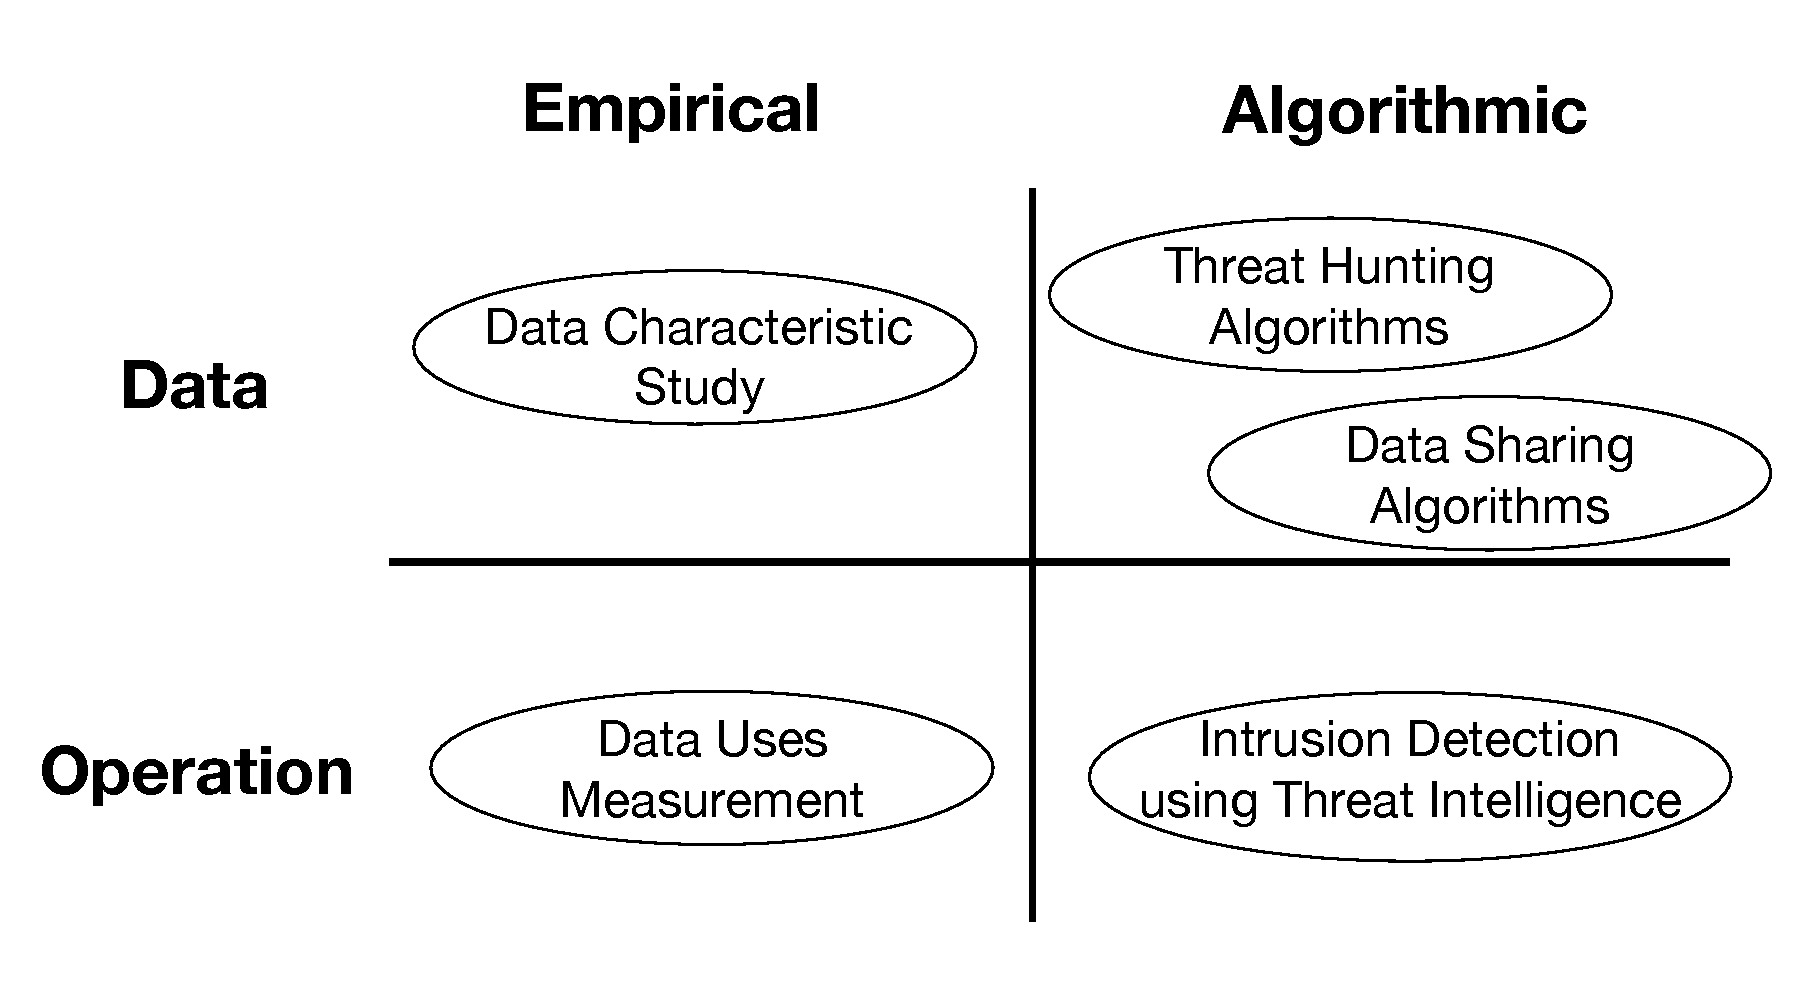
\includegraphics[width=0.8\textwidth]{threat_intel_research_overview.pdf}
\caption{Threat Intelligence research overview and example research
topics in each direction.}
\label{fig:threat_intel_overview}
\end{figure}

Therefore, research directions related to Threat Intelligence can be 
viewed in four general categories, as illustrated in
Figure~\ref{fig:threat_intel_overview}. More specifically, the four 
research directions are: 
\begin{prettylist}
    \item Empirical analysis on Threat Intelligence data: \\
    Understanding the characteristic of Threat Intelligence data, different
    data generation systems and their performance, different threat sharing
    strategies and how are they being used in the real-world, etc.
    
    \item Algorithm exploration related to Threat Intelligence data: \\
    Designing algorithms for threat hunting (Threat Intelligence generation),
    specification for data description and protocols for data sharing, etc.
    
    \item Empirical analysis on Threat Intelligence usage: \\
    Measuring how organizations are using Threat Intelligence, the problems 
    when using these data and the impact on the Internet, etc.
    
    \item Algorithm exploration related to Threat Intelligence usages: \\
    Designing better methods to use threat intelligence during system and 
    network defense(e.g. increasing coverage, reducing false positives),
    explore new ways to use threat intelligence data, such as using the 
    data as machine learning training data, etc.
\end{prettylist}

In this dissertation, I take an empirical approach and explore the 
\textit{Data} and \textit{Operation} problems of Threat Intelligence.
I focus on thoroughly understanding the current status of Threat 
Intelligence and will then discuss my takeaways from these analyses.
In the study of \textit{Data}, which will be discussed in Chapter~\ref{chapter:data_character}, 
I analyzed the data characteristics of existing Threat Intelligence products.
I designed mathematics metrics for Threat Intelligence data evaluation,
and with these metrics, I studied \numipfeeds\ distinct IP address 
data feeds, covering six categories of threats, and \numhashfeeds\ distinct
malware file hash feeds, and measured their data characteristic. Through this
work, I revealed the limitation of existing Threat Intelligence data and 
discussed the potential improvements based on my findings. In the study of
\textit{Operation}, which will be discussed in Chapter~\ref{chapter:data_usage},
I measured how Threat Intelligence data is being used on a large scale. 
I designed a method using IP ID side channel that can measure the 
connectivity between two Internet hosts from a third point. With this 
method, I conducted a large scale Internet measurement over {\reflroughnum} 
U.S. hosts and uncovered their uses of {\blacklistnum} popular public IP
blacklists. I further investigated a broader use of blacklists among the 
hosts, and discovered over 73K hosts has shown blacklist related blocking 
behavior. Together, my work provided an in-depth look into the current
status of Threat Intelligence and augmented the knowledge of our community
on this topic.

%\verb!\mainmatter! macro because it should start on page~1.
%\end{dissertationintroduction}

\chapter{Background}
\label{chapter:background}

\section{Threat Hunting}
\subsection{Intrusion Detection}

One direct way to capture threat is to identify the attacker when a
system in use is under attack, so we can capture the 
attacker in action. These systems can be specially deployed systems
just for luring attackers, like honeypot; they can also be real systems
with real users, where people deploy detection system and capture 
attacks when they are happening. The technique we use here is also 
the technique to protect the system in the first place:
\textit{Intrusion Detection}.

Intrusion detection aims to detect attacks on network or system on the
fly. The techniques involved can generally be classified as two 
categories: misuse-based detection and anomaly-based detection.
Misuse-based approaches utilize pre-defined patterns and signatures
of malicious behaviors, and dynamically compare the behavior of the
system against these patterns to spot potential intrusion. On the another
hand, anomaly-based detection construct a model for the normal behavior 
of a system, then check if the current behavior is deviating from the 
``normal'' behavior.

The performance of misuse-based detection methods depends on the quality
of the pre-defined attack patterns (or detect policies), and these 
patterns are usually provided manually by security experts. Since 
different attack vectors vary a lot on their approaches and system 
component they touch, the 
patterns provided by the detection system must be able to cover a 
diverse set of behavior, also to be extendable, as new attacking
methods are keep showing up. Therefore, early work on this technique like
Bro~\cite{paxson1999bro}, Snort~\cite{roesch1999snort}, 
P-BEST~\cite{lindqvist1999detecting}, and STAT~\cite{vigna2003designing}
all emphasize on the providing a powerful threat modeling language, which
can express a broad set of threat, also easy to program to include new 
patterns. Recent works like~\cite{bugiel2012towards} move to new
system environment (e.g. mobile system like Android), but still focus
on providing a expressive modeling language to build detect policies. 
These misuse-based detection methods is generally accurate, since the
pre-defined attack patterns are usually well defined by security experts. 
The main disadvantage of this technique is that it can only detect 
modeled attacks. For new type of attacks where there are no pattern
written, misuse-based system will miss them completely.

As a complementary, anomaly-based detection methods try to detect if
the behavior of an application or system is different from its benign
behaviors. This technique relies on modeling the normal behavior of a 
system in question, and since there are so many possible things a program 
can do, we need to simplify the ``behavior'' to precisely reason about 
it. Forrest et. al.~\cite{forrest1996sense} first proposed to use
syscall sequence of a program as its behavior, since a program can only
affect the operating system with syscalls, and from the security 
perspective, these would be the only behaviors that matters. Follow up
works like ~\cite{lee1998data, warrender1999detecting, mutz2006anomalous}
explored different data model to better distinguish abnormal sequences
from benign ones, using method like data mining, Bayesian network and 
neural network. Recent works like~\cite{du2017deeplog} also try to 
utilize more data sources and experiment with more advanced machine
learning algorithm for the detection. The advantage of these approaches 
is that it can capture previously unknown attacks. However, it tends
to suffer more false positives, since a normal program can show abnormal
behaviors once a long while, and it is very hard to capture these
cases when we first build the ``normal'' behavior set for a program.

\subsection{Causality Analysis}
Intrusion detection techniques described before detects threats 
when abnormal behavior is observed. But for many advanced 
attacks, especially the APTs(Advanced Persistent Threats), it 
is not always obvious to trace from the malicious behavior, e.g.
a running malware, to the source of the attacks, e.g. a phish 
URL that distributes the malware. This is mainly because sophisticated
attacks often take precautions to hide their traces by deleting
system or application logs, they can also prolong the attacks, 
creating a large window from the time they break into victims' 
machines till the time they actually carry out malicious activities. 
All of these can create difficulties for administrators to diagnose
the intrusion and trace the source. In the context of Threat 
Intelligence, it is important to uncover the source of 
an attack, so we can provide valuable indicator-of-compromise for the 
community to defense the same attack in an early stage.

The analysis, which tracks causal relationships between files and 
processes to diagnose attack provenances and consequences, is called
\textit{Attack Causality Analysis}. It is an critical technique
during threat intelligence hunting. The pioneering work in this field
is done by King and Chen~\cite{king2003backtracking}. They first defined
the event dependency graph, where the nodes represent processes and files
and edges represent the events between process and files, for example,
a process spawn another process, or a process read or write to a 
file. Given a detection point, like a suspicious files or a running
process, the system builds a dependency graph from this points by
processing event logs, then using the timestamp of each events and 
their causal relationship, we can trace back to the source and identify
the original intrusion point.

A simple idea as it seems, it captured the fundamental logic behind 
causality analysis: information flow tracking. However, this simple
solution quickly runs into a problem in a complex system: 
\textit{dependence explosion}~\cite{goel2005taser}, where there are 
so many processes and files involved in this dependency graph, together
with large amount inter-relations, that it is very hard identify the
real attack from the haystack. The case become even more true when there
are long-running programs, like a server program. The dependency 
associated with these program will grow enormously over 
time~\cite{lee2013high}, making the dependency graph even more 
complicated.

Many work have tried to tackle this problem. Some heuristics have been 
proposed to prune the graph, like in~\cite{king2005enriching}, the 
authors utilized the fact that worms try to exploit from host to host,
so the traffic from a host who already has an IDS alert is more likely
associated with worm attacks. Liu et al.~\cite{liu2018towards} uses
the rareness of events as a metric to prioritize searching on dependency
graphs. Other work try to break the entities on the graph into smaller 
granularity, so we can pinpoint the causal relationship between objects.
For example, Goel et al.~\cite{goel2005taser} use the separate socket
reads to partition the execution of a program into different segments, 
so the monitoring system can figure out which action of that program
is corresponded with which exact network request. Lee et 
al.~\cite{lee2013high} use the prevalence of event-loops in programs to
partition the execution of the program based on each loop iteration,
and then associates events with specific loop iterations. Binary taint
tracking has also been utilize to provide richer semantic information, 
like demonstrated in~\cite{ma2016protracer}. This topic is still an 
active topic today and researcher are trying to solve this from different
angle.
\subsection{Malware Analysis}
Malicious software, often called malware, is always a pressing threat 
on the Internet. It has been used by attackers to steal sensitive user data, 
control victim machines to launch spam campaigns or DDoS campaigns, or 
encrypt valuable data to demand ransom, etc. Symantec has reported over 200 
Million new malware variants just in 2018 alone~\cite{symantecmalware}. 
Therefore, it is crucial for threat intelligence products to cover recent 
malware comprehensively.
Malware threat intelligence data usually comes as two forms: file hashes,
like MD5, that represent malware variants themselves, and IPs or domains
that host Command-and-Control servers for the malware. Both forms of 
data is critical for organizations, as the presence of either form 
indicates a strong possibility of compromise, and immediate actions need 
to be taken. To generate these data, security companies rely on analyzing 
unknown binaries, collected from the Internet or uploaded by customers,
to determine if they are malicious.

To identify if an unknown binary is malware, one straightforward yet
effective way is to check if the binary is a variant of known malware.
Since it is nontrivial to develop a sophisticated malware program, 
attackers tend to just modify existing malware to generate new unseen
variants. Some typical ways include code transformation(e.g. replace ``mov 
eax, 0'' with ``xor eax, eax''), obfuscation, or encrypting the original 
binary and stores the result as data in a new executable (with a packer 
program). These simple techniques enable attackers to quickly generate a 
large number of variants from a single malware instance, and significantly 
increase the overhead for security experts to analyze them.

To compare a new malware sample with existing ones, we need to define a 
suitable representation of malware samples, from which we can calculate 
the similarity between them. There are two approaches to construct this 
``representation'': \textit{Content-based} and \textit{Behavior-based}. 
Content-based approach abstracts a program based on its code content, and 
calculate the similarity between programs by comparing their code. 
Early work by M. Gheorghescu~\cite{Gheorghescu2006ANAV} propose 
to break the malware program into basic blocks and compare the similarity 
between those blocks.
Dullien et al.~\cite{dullien2005graph} extract control flow graphs from 
malware programs and use graph similarity as the similarity between programs.
These content-based approaches rely on analyzing program code itself, so 
they still suffer the problem of advanced code obfuscation, which can modify
the code dramatically while maintaining the same functionality. This leads to
the behavior-
based approach, where we extract the actual behavior of malware and use that
as the signature for comparison. Lee et al.~\cite{lee2006behavioral} propose
to use system call sequence as the signature to classify different malware
samples. Bailey et al.~\cite{bailey2007automated} use the \textit{non-transient
state changes} malware causes on a system(files written, processes created) as 
the behavior signature, and do the comparison based on these behaviors. Holz 
et al.~\cite{rieck2008learning} further developed this behavior-based method, 
and use the actions of malware as machine learning features, and use a 
supervised machine learning model to conduct the comparison and classification.
Bayer at al.~\cite{bayer2009scalable} used taint tracking to capture a finer
granularity of malware's behavior, and use this information for more precise
identification. The behavior-based approaches usually capture the behavior of
malware through dynamically executing the malware samples, so it won't be 
affected by malware code itself, but executing the code for every variant in
question impose nontrivial overhead. 

When there is no existing malware to compare with, or the program in question 
does not match any known malware, an analysis system will need to decide if
the program is malicious just based on the behavior of the program itself. Like
the intrusion detection methods described in the previous section, the logic
here also relies on having ``specifications'' that cover potential malware 
behaviors, and check if the analyzed program exhibits those behaviors. One 
common heuristic is to check if the program makes any changes to the system
registry. GateKeeper~\cite{wang2004gatekeeper}, for example, detect spyware
by monitoring if the program register as an OS auto-start extension, such as 
an NT service, a tray icon in Windows, or a Unix daemon/cron job. Other tools
also check different detection points, like VICE~\cite{bulter2004vice}, which
checks for the existence of various hooks used by rootkits. More advanced 
systems tend to further monitor the detailed behavior of the program, like 
in~\cite{kirda2006behavior}, the authors try to detect a popular type of
spyware that uses Internet Explorer’s Browser Helper Object (BHO) and 
toolbar interfaces to monitor a user’s browsing behavior. The system uses 
dynamic analysis to track if the program monitors users' actions and sends
out its findings to an external entity. Panorama~\cite{yin2007panorama}, 
similarly, use dynamic taint tracking to construct the information flow of
an unknown program, and then use pre-defined policies(specifications) to 
determine if the program is malicious or not.

\subsection{Spam Detection}
Spam email, also referred as unsolicited bulk email or junk mail, is 
Internet mail that is sent to a group of recipients who have no intention 
to receive it. They are particularly harmful, as these emails jams users' 
mailboxes, engulf important personal mail, waste network bandwidth and 
can even crash mail-servers. Spam emails also serve as an important
way of advertising products in underground market, like prescription drugs, 
illegal porn, replica of other brands etc. It is an old yet still popular
threat on the Internet. Threat Intelligence spam data contains domains, 
from which spammers send the spam email, and IP addresses, where spammers' 
mail servers are located. Organizations, and even ISPs, tend to use these 
data to block the incoming mail traffic.

Email providers, ISPs or anti-spam organizations usually set up 
\textit{Spamtrap} to capture spam emails. Spamtrap are the email addresses
that are created not for communication, but rather to lure spam. These
email addresses do not belong to any person and will not involve in any
kind of communication. These addresses will not be revealed openly online,
so only unsolicited spammers, who tend to collect target email addresses
by crawling the Internet, or go through all possible lexical combinations
for email names, will hit these addresses. The Spamtrap here serve as a 
bait to capture spammers. People also recycle long out-of-date email 
addresses as Spamtrap addresses. 

However, simply regarding all emails received in Spamtrap as spam emails 
will create a substantial amount of false positives, since legitimate senders with poor data hygiene or acquisition practices end up hit the traps as 
well. To further distinguish spam emails and consequently identify the
senders, one needs to look at the content of emails themselves. Numerous 
statistical algorithms have been proposed by researchers to filter spam
emails from legitimate ones. At its core, spam filtering can be viewed as
a text categorization task: given the full text content of an email, 
decide whether it is spam email or benign email. A variety of supervised
machine learning techniques have been tested for spam filtering. Like the
naive Bayes classifier~\cite{androutsopoulos2000evaluation, sahami1998bayesian, schneider2003comparison}, 
RIPPER rule induction algorithm~\cite{cohen1996learning},
Support Vector Machine~\cite{drucker1999support}, memory-based learning
~\cite{androutsopoulos2000learning}, AdaBoost~\cite{carreras2001boosting},
and maximum entropy model~\cite{zhang2003filtering}. These algorithms all
convert email headers and body into features for the machine learning model,
and different feature reduction and weight assignment strategy have been
explored. These models can all achieve decent accuracy, and have been tested
and deployed in real-world. 

Email providers also get help from the customers to identify spams. Since
customers can mark an email as spam manually, having a large customer base
enables the email provider to collect a large amount of spam emails with high
accuracy, and therefore track down the domains and IP addresses used by the 
spammers.

\subsection{Phishing Detection}
\textbf{TODO}



\section{Threat Intelligence Specifications and Sharing Systems}
\textbf{TODO}

\section{Threat Intelligence Data Analysis}

Several studies have examined the effectiveness of blacklist-based 
threat intelligence~\cite{kuhrer2014paint, ramachandran2006revealing, 
ramachandran2007filtering, sheng2009empirical, sinha2008shades}.
Ramachandran~\etal~\cite{ramachandran2007filtering} showed that spam 
blacklists are both incomplete (missing 35\% of the source IPs of 
spam emails captured in two spam traps), and slow in responding 
(20\% of the spammers remain unlisted after 30 days).
Sinha~\etal~\cite{sinha2008shades} further confirmed this result by 
showing that four major spam blacklists have very high false negative
rates, and analyzed the possible causes of the low coverage.
Sheng~\etal~\cite{sheng2009empirical} studied the effectiveness of
phishing blacklists, showing the lists are slow in reacting to
highly transient phishing campaigns.

Other studies have analyzed the general attributes of threat
intelligence data. Pitsillidis~\etal~\cite{tasters:imc12} studied the
characteristics of spam domain feeds, showing different perspectives
of spam feeds, and demonstrated that different feeds are suitable for
answering different questions. Thomas~\etal~\cite{thomas2016abuse}
constructed their own threat intelligence by aggregating the abuse
traffic received from six Google services, showing a lack of
intersection and correlation among these different sources. 

The limitations of the previous measurement works are that these 
studies tend to only focused on specific types of threat intelligence 
sources, like spam or phish blacklists, and they only evaluated one 
aspect of the data characteristic, like the operational performance, 
rather than generalize the measurement and define threat intelligence 
metrics that can be extended beyond the work.

Little work before had defines a general measurement methodology to
examine threat intelligence across a broad set of types and categories.
Metcalf~\etal~\cite{metcalf2015blacklist} collected and measured IP
and domain blacklists from multiple sources, but again only focused 
on volume and intersection analysis. One missing piece in these works
is that they did not approach the problem from the perspective of 
consumers of Threat Intelligence.  After all, it is the consumers that
will support this industry, and research communities should look more
into their needs. This is one major motivation of my work, which will
be discussed in Chapter~\ref{chapter:data_character}.
\section{Threat Intelligence Uses}
\label{sec:threat_intel_uses}

Threat intelligence data, at a high-level, promises that by compiling up-to-date 
information about known threats (i.e., IP addresses, domain names, file hashes, 
etc.), recipients of the data will be able to better defend their systems from 
future attacks. Therefore, the primary use cases of threat intelligence is 
network defense. Intrusion detection systems or firewalls can directly put 
the data in the system and block the corresponding IP or DNS traffic. Popular 
open source projects like Snort~\cite{snortids}, Zeek~\cite{zeekids} all provide 
these functionalities. Commercial products like Palo Alto Network
firewall~\cite{paloaltofirewall}, Fortinet firewall~\cite{fortinetfirewall}, 
Cisco firewall~\cite{ciscofirewall} also incorporate threat intelligence data in 
their defense systems. 

Besides directly taking action, threat intelligence can also be used in security
monitoring and post forensic analysis. In these cases, the system raises alarms
when there are matches between network activities and threat intelligence data.
Threat intelligence data usually come with confidence and severity level for each
individual data item. When investigating these alarms, administrators can 
prioritize the investigation based on the severity level. The system that in 
charge of collecting and organization security alarms are called Security 
Information and Event Management system, or SIEM system. Popular SIEM systems
include Splunk~\cite{splunk}, Sumo Logic~\cite{sumologic} and LogRhythm NextGen 
SIEM~\cite{logrhythm} etc.

In academic research, threat intelligence data is usually used as extra source 
data to assist their study, or to evaluate the performance of their systems or
algorithms. For example, Hao et. al.~\cite{hao2016predator} explored using the
characteristic domains during domain registration to detect potential malicious
domains. In the study, the authors use Spamhaus domain blacklist, URIBL to check 
the accuracy of their prediction. Singh et. al.~\cite{singh2017characterizing} 
studied the characteristic of Tor exit blocking in the wild, and use public and
private threat intelligence sources to see how much of Tor exit IPs are listed
on these sources. These are experimental use cases researchers have explored 
with threat intelligence data. 

One question that has not been investigated is how threat intelligence 
products are actually being used by organizations currently in the industry.
Understanding the real-world use cases gives us ideas about the adoption of threat
intelligence data, which is essential information to know in the threat
intelligence ecosystem. More importantly, the usage of different products offers
us insight into the potential impact they could cost on the Internet. As 
discussed in Chapter~\ref{chapter:data_character}, false positives are relatively 
common in threat intelligence feeds. If an organization is using one threat
intelligence IP feed in its firewall for IP-based traffic blocking, and there
is a false positive(a benign IP address) in this feed, then all the users in
that organization will be affected. From another side, if one online host is
added to an IP feed mistakenly, then this host will lose access to all the
organizations that use this feed as a blocking ruleset. Therefore, the actual
usage of the data in industry is a crucial topic that should get more attention
from the security community.

But this problem is also a very challenging problem. The primary challenge 
is that there are many ways people can use these data. It can be directly 
used to block network traffic, or just raise an alarm in their Security
Information and Event Management(SIEM) systems. Some use cases do not even 
have a well-defined behavior that we can quantitatively measure. 
The actions derived from threat intelligence data can also happen at different
network layers. For example, an organization can deny access on network layer; 
it can also deny access on application layer, like HTTP 403 Forbidden. 
This diverse possibility of use cases makes it hard to assess this problem as 
a whole. 

Little work has been done to try and understand how threat
intelligence data is being used on a large scale. The only work that tries to
look at threat intelligence data from this perspective are industrial surveys
-- wherein organizations fill out questionnaires. One such survey conducted by
the Ponemon Institute~\cite{ponemon2018cti}, surveyed 1,200 IT and IT
security practitioners, asking if they use threat intelligence products, and
if they do what tools do they use that utilize the threat intelligence data.
The survey also asked their user experience. SANS Institute did a
similar study~\cite{shackleford2017cyber} where they surveyed 600
participants from a diverse industry background and asked questions about
their threat intelligence usage. These works are limited in terms
of scale, and their results are all at a very high-level. Although they offered
some useful insight, they can not provide us a concrete understanding
of threat intelligence uses on a large scale. My measurement,
which will be discussed in Chapter~\ref{chapter:data_usage},
is the first work that systematically looks at the problem of inferring
threat intelligence uses and explore its implications.


\chapter{An ordinary page}
The purpose of this page is to illustrate an ordinary page of text in
a doctoral dissertation or master's thesis. All pages of the doctoral
dissertation or master's thesis must be kept within the margins of
1.5'' on the left, 1'' on the right, 1'' on the top and 1.25'' on the
bottom. All text must be double spaced except as indicated below.

It is recommended that to increase the margins as paper can shift in a
printer and as some photocopiers tend to increase the image being
copied.

The first line of each paragraph must be indented at least one 0.5''
tab, as done here.

This text is intended to be a part of the dissertation, for a doctoral
student, or the thesis if you are receiving a master's degree, and now
a quote is included here:
\begin{quote}
All quotes of more than six lines, even though this one is not, are to
be indented 0.5'' from the left and 0.5'' from the right. These longer
quotes are to be single spaced. Don't forget to adjust for proper
spacing after the last line of the quoted material.
\end{quote}
The rest of the paragraph would continue as so.

\chapter{Figures and Such}
This demonstrates how OGS wants figures and tables formatted. For
figures, the caption goes below the figure and ``Figure'' is in bold.
See Figure~\ref{fig:zen}. Tables are formatted with the caption above
the table. See Table~\ref{tab:bad}.

Of course, Table~\ref{tab:bad} looks horrible. It should probably be
formatted like Table~\ref{tab:good} instead.

For facing caption pages, see Table~\ref{tab:facing}. Of course,
facing caption pages are vaguely ridiculous and my implementation of
them in the class file is by far the most brittle part of the
implementation. It's entirely possible that something has changed and
these don't work at all. I implemented it merely for the challenge.

\begin{figure}
\centering
\fbox{\parbox{.9\linewidth}{%
	\noindent
	{\Huge PHD ZEN}\par
	\vskip.5in
	\centerline{comic here}
	\vskip.5in
}}
\caption[``Ph.D. Zen'']{Comic entitled ``Ph.D. Zen'' by Jorge Cham, 2005. Copyright
has not been obtained and so it isn't displayed.}
\label{fig:zen}
\end{figure}

\begin{table}
\centering
\caption[Electronic Dissertation Submission Rates]{Electronic
Dissertation Submission Rates at UCSD, Fall 2005 and Winter 2006.
(First two quarters that the program was available to all Ph.D.
candidates not in a Joint Doctoral Program with SDSU.)}
\label{tab:bad}
\begin{tabular}{|*{5}{>{\centering\arraybackslash}m{.15\linewidth}|}}
\hline
&Ph.D.s awarded (Including Joint degrees) & Electronic submission of
Dissertation & Paper Submission of Dissertation & Percentage of
Electronic Submission\\
\hline
Fall\par 2005 & 84 & 37 & 47 & 44.05\%\\
\hline
Winter\par 2006 & 64 & 42 & 22 & 65.63\%\\
\hline
\end{tabular}
\end{table}

\begin{table}
\centering
\caption[Electronic Dissertation Submission Rates]{Electronic
Dissertation Submission Rates at UCSD, Fall 2005 and Winter 2006.
(First two quarters that the program was available to all Ph.D.
candidates not in a Joint Doctoral Program with SDSU.)}
\label{tab:good}
\renewcommand\tabularxcolumn[1]{>{\RaggedRight\arraybackslash}p{#1}}
\begin{tabularx}{.9\linewidth}{lcccc}
\toprule
&\multicolumn{1}{X}{Ph.D.s awarded (Including Joint degrees)}
&\multicolumn{1}{X}{Electronic submission of Dissertation}
&\multicolumn{1}{X}{Paper Submission of Dissertation}
&\multicolumn{1}{X}{Percentage of Electronic Submission}\\
\midrule
Fall 2005 & 84 & 37 & 47 & 44.05\%\\
Winter 2006 & 64 & 42 & 22 & 65.63\%\\
\bottomrule
\end{tabularx}
\end{table}

\begin{facingcaption}{table}
\caption[UCSD Gender Distribution]{University of
California, San Diego Gender Distribution for the Campus Population,
October~2005\\
(http://assp.ucsd.edu/analytical/Campus\%20Population.shtml)\\
\emph{(This is an example of a facing caption page, the next page is
the example of the table/figure/etc.\ that corresponds to this
caption. It is also an example of table/figure that is rotated 90
degrees to fit the page.)}}
\label{tab:facing}
\renewcommand\tabularxcolumn[1]{>{\RaggedLeft\arraybackslash}p{#1}}
\parindent=0pt
\setbox0=\vbox}
& \multicolumn{1}{c}{\textbf{N}} & \multicolumn{1}{c}{\textbf{\%}}
& \multicolumn{1}{c}{\textbf{N}} & \multicolumn{1}{c}{\textbf{\%}}\\
\midrule
Students & 12,987 & 51\% & 12,686 & 49\% & 25,673 & 100\%\\
Employees & 9,943 & 56\% &  7,671 & 44\% & 17,614 & 100\%\\
\addlinespace
\hfill\textbf{Total} & \textbf{22,930} & \textbf{53\%} &
\textbf{20,357} & \textbf{47\%} & \textbf{43,287} & \textbf{100\%}\\
\bottomrule
\end{tabularx}
\singlespacing

\emph{Notes}:
\begin{enumerate}
\item The counts shown below will differ from the official quarterly
Registrar's registration report because 1) data for residents in the
Schools of Medicine and Pharmacy and Pharmaceutical Science are
excluded, and 2) registered, non-matriculated, visiting students are
included.
\item Student workers are excluded from employees; however emeritus
faculty and others on recall status are included.
\end{enumerate}

Campus Planning. Analytical Studies and Space Planning\\
31 January 2006
}
\centerline{\rotatebox{90}{\box0}}
\end{facingcaption}

% This will give us some more text
\Blinddocument

% Skipping a bunch of chapters
\setcounter{chapter}{50}
\chapter{Another chapter}
\setcounter{figure}{73}
\setcounter{table}{88}
\begin{figure}
\centering
\fbox{\hbox to.8\linewidth{\hss Another figure\hss}}
\caption{Another figure caption}
\end{figure}
\begin{table}
\centering
\caption{Another table caption}
\begin{tabular}{ccc}
\toprule
X&Y&Z\\
\midrule
a&b&c\\
\bottomrule
\end{tabular}
\end{table}
\begin{figure}
\caption{ASDF fig}
\end{figure}
\begin{table}
\caption{ASDF tab}
\end{table}

\appendix
\Blinddocument

% Stuff at the end of the dissertation goes in the back matter
\backmatter
\bibliographystyle{plain} % Or whatever style you want like plainnat
\bibliography{references}

\end{document}
